\section{SVM}

\begin{frame}{Support Vector Machine(a.k.a. SVM)}

\begin{itemize}
    \item 支持向量机是一种监督学习算法
    \item 通过构造极大边距超平面以更好泛化
    \item 两种常见形式:Hard-SVM 和 Soft-SVM
\end{itemize}
\end{frame}

\begin{frame}[fragile]{Hard-SVM}
    \begin{itemize}
        \item 设训练数据集 $S=\left\{ (\mathbf x_1, y_1), (\mathbf x_2, y_2), \cdots, (\mathbf x_m, y_m) \right\} $ ,其中$\mathbf x_i \in \mathbb R^d$,$y_i \in \left\{ -1, 1 \right\} $。
        \item 线性可分数据集:存在一个超平面 $(\mathbf w, b)$ 使 $\forall i, y_i = \text{sign}(\left\langle \mathbf w , \mathbf x_i \right\rangle +b )$。
        \item Hard-SVM 只能处理线性可分数据集。
    \end{itemize}
    算法:
    \begin{center}
        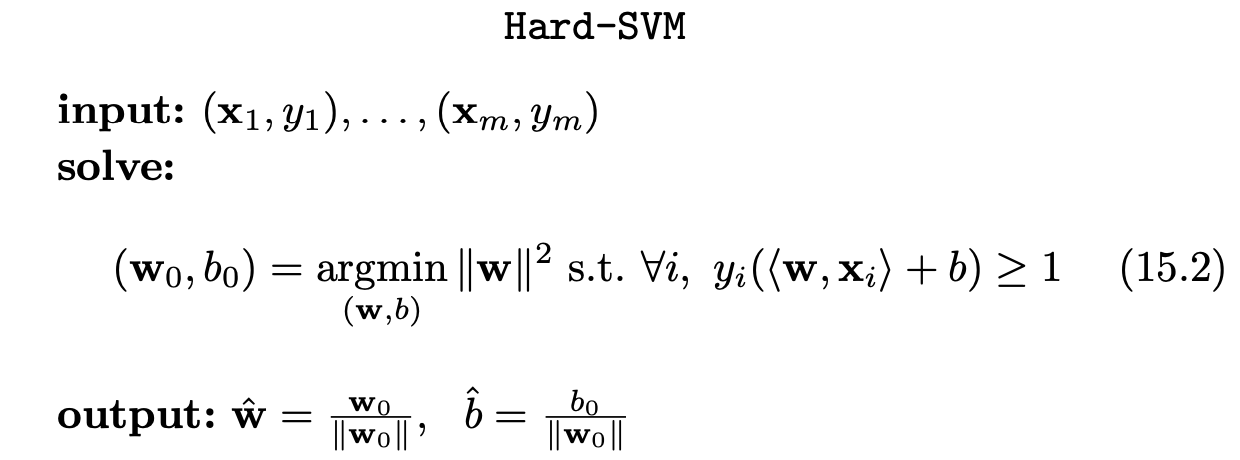
\includegraphics[width=0.6\textwidth]{assets/hsvm.png}
    \end{center}
    分析:固定标度最大化边距,相当于固定边距最小化标度;最后归一化还原成固定标度最大化边距的结果。
    
\end{frame}

\begin{frame}[fragile]{Soft-SVM}
    \begin{itemize}
        \item Soft-SVM 可以处理非线性可分数据集。
        \item 思想:放宽限制为 $y_i (\left\langle \mathbf{w}, \mathbf{x}_i \right\rangle + b) \geqslant 1-\xi_i$
    \end{itemize}
    算法:
    \begin{center}
        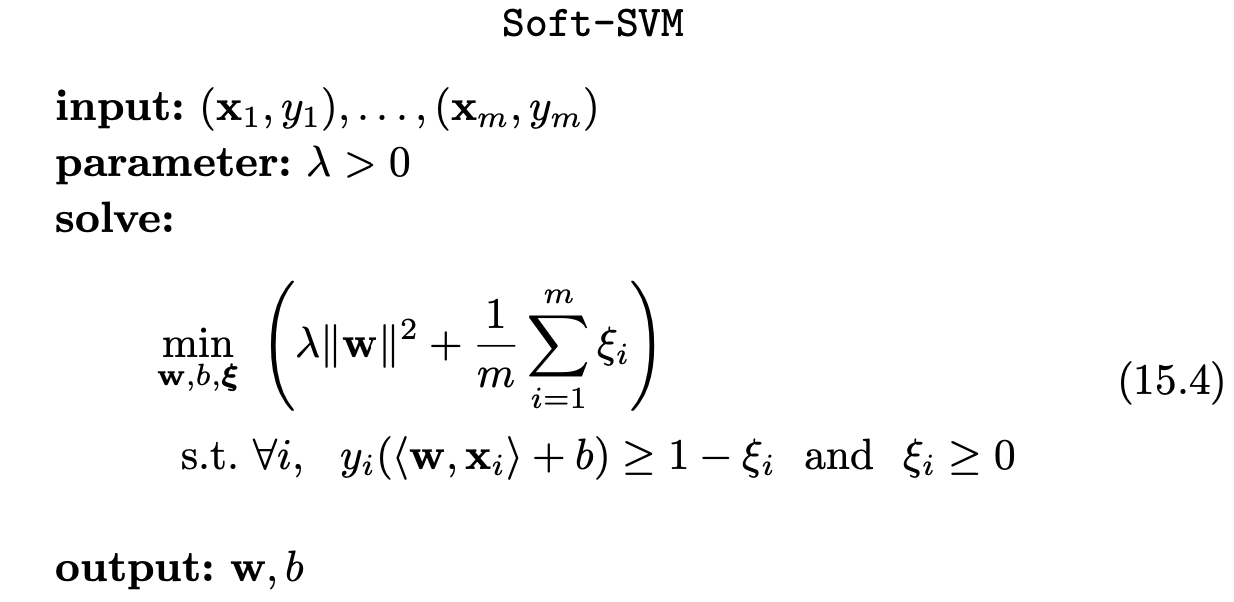
\includegraphics[width=0.6\textwidth]{assets/ssvm.png}
    \end{center}
    
\end{frame}

\begin{frame}[fragile]{hinge loss}
    \begin{itemize}
        \item 定义 hinge loss $\ell^{\text{hinge}}(x) =\max \left\{ 0, 1-x \right\}  $
        \item 定义 $L_S^{\text{hinge}}((\mathbf{w}, b)) = \frac{1}{m}\sum_{i=1}^{m} \ell^{\text{hinge}}(y_i\cdot(\left\langle \mathbf{w}, \mathbf{x}_i \right\rangle + b))$
        \item 注意到 (15.4) 式等价于
        \[
           \min_{\mathbf{w}, b} \left( \lambda \left\| \mathbf{w} \right\|^{2} + L_S^{\text{hinge}}((\mathbf{w}, b))  \right) 
        \]
        这就是标准的 regularized loss minimization problem,其中 $\lambda \left\| \mathbf{w} \right\|^{2}$ 是 $\ell_2$ 正则化。
        \item 因此 Soft-SVM 等价于一个hinge loss、$\ell_2$正则化的优化问题。
    \end{itemize}
\end{frame}

\begin{frame}[fragile]{duality}
    \begin{itemize}
        \item 以 Hard-SVM 为例(忽略$b$),定义
        \[
            g(\mathbf{w}) =\max_{\mathbf\alpha\in \mathbb{R}^{m},\mathbf \alpha \geqslant 0} \sum_{i=1}^{m} \alpha_i \cdot (1- y_i \cdot (\left\langle \mathbf{w}, \mathbf{x}_i \right\rangle)) = \begin{cases} 0 &\text{if }\forall i, y_i\left\langle \mathbf{w}, \mathbf{x}_i \right\rangle \geqslant 1   \\ +\infty & \text{otherwise} \end{cases}
        \]
        则(15.2) 式等价于
        \begin{align*}
            &\min_{\mathbf{w}} \left( \left\| \mathbf{w} \right\|^{2} + g(\mathbf{w})  \right)  \\
            = & \min_{\mathbf{w}} \max_{\mathbf\alpha\in \mathbb{R}^{m}, \mathbf\alpha \geqslant 0} \left( \left\| \mathbf{w} \right\|^{2} + \sum_{i=1}^{m} \alpha_i \cdot (1- y_i \cdot (\left\langle \mathbf{w}, \mathbf{x}_i \right\rangle))  \right) = p^{*} \\
            \geqslant & \max_{\mathbf\alpha\in \mathbb{R}^{m}, \mathbf\alpha \geqslant 0} \min_{\mathbf{w}} \left( \left\| \mathbf{w} \right\|^{2} + \sum_{i=1}^{m} \alpha_i \cdot (1- y_i \cdot (\left\langle \mathbf{w}, \mathbf{x}_i \right\rangle))  \right) = d^{*} \tag{1}
        \end{align*}

        \item 在Hard-SVM中,由于特殊条件的满足,$p^{*} = d^{*}$,所以可以通过求解对偶问题来求解原问题。
    \end{itemize}
\end{frame}

\begin{frame}[fragile]{duality}
    \begin{itemize}
        \item 对内部 $\mathbf{w}$ 取最小值,得到 $\mathbf{w} = \sum_{i=1}^{m} \alpha_i y_i \mathbf{x}_i$
        \item 带回对偶问题$(1)$式,得到 
        \[
            \max_{\mathbf\alpha\in \mathbb{R}^{m}, \mathbf\alpha \geqslant 0} \left( \sum_{i=1}^{m} \alpha_i - \frac{1}{2} \sum_{i=1}^{m} \sum_{j=1}^{m} \alpha_i \alpha_j y_i y_j \left\langle \mathbf{x}_i, \mathbf{x}_j \right\rangle  \right)
        \]
        \item 关键:只与 $\left\langle \mathbf{x}_i, \mathbf{x}_j \right\rangle$ 有关,而不与 $\mathbf{x}_i$ 有关,这是核技巧的基础。
    \end{itemize}
\end{frame}

\begin{frame}[fragile]{kernel method}
    \begin{itemize}
        \item 思想:由于很多问题在原空间中线形不可分,希望先将原数据点映射到一个(更高维)空间中,然后在更高维空间中执行SVM算法。
        \item 算法:
        \begin{itemize}
            \item 设原数据点定义域为$X$, 映射函数为 $\phi: X \to F$,其中 $F$ 是特征空间(feature space)。
            \item 给定原带标签数据集 $S=\left\{ (\mathbf x_1, y_1), (\mathbf x_2, y_2), \cdots, (\mathbf x_m, y_m) \right\} $,构造像数据集 $\hat S = \left\{ (\phi(\mathbf x_1), y_1), (\phi(\mathbf x_2), y_2), \cdots, (\phi(\mathbf x_m), y_m) \right\} $。
            \item 在$\hat S$上执行SVM算法,得到超平面 $(\mathbf w, b)$,对应一个线性分类器$h: \psi(\mathbf{x}) \mapsto y$。
            \item 预测原空间中test set example $\mathbf{x}$ 为 $h(\psi(\mathbf{x}))$
        \end{itemize}
    \end{itemize}
\end{frame}

\begin{frame}[fragile]{kernel}
    \begin{itemize}
        \item kernel 是 feature space 中的 inner product。
        \item 给定 embedding $\phi: X \mapsto F$, 定义 kernel function 
        \[
            K(\mathbf{x}, \mathbf{x'}) = \left\langle \phi(\mathbf{x}), \phi(\mathbf{x'}) \right\rangle
        \]
        \item $K$ 表征了$\mathbf{x}, \mathbf{x'}$ 的相似度
    \end{itemize}
\end{frame}

\begin{frame}[fragile]{kernel trick}
    \begin{itemize}
        \item 很多SVM问题都可以总结为以下 general 问题的实例:
        \[
           \min_{\mathbf{w}} \left( f(\left\langle \mathbf{w}, \mathbf{x}_1 \right\rangle, \left\langle \mathbf{w}, \mathbf{x}_2 \right\rangle, \cdots, \left\langle \mathbf{w}, \mathbf{x}_m \right\rangle ) + R(\left\| \mathbf{w} \right\|_2 )\right) 
        \]
        \item Example 1: Soft-SVM, $R(a) = \lambda a^{2}$, $f(a_1, a_2, \cdots, a_m) = \frac{1}{m} \sum_{i=1}^{m}\max \left\{ 0, 1-y_i a_i \right\} $
        \item Example 2: Hard-SVM, $R(a) = a^{2}$, $f(a_1, a_2, \cdots, a_m) = \begin{cases} 0 & \text{if } \exists  b \text{ s.t. } y_i (a_i+b) \geqslant 1 \\ +\infty & \text{otherwise} \end{cases} $
        \item 而 $\mathbf{w} \in \text{span}(\mathbf{x}_1, \mathbf{x}_2, \cdots, \mathbf{x}_m)$(\href{https://www.cs.huji.ac.il/w~shais/UnderstandingMachineLearning/understanding-machine-learning-theory-algorithms.pdf}{\underline{reference}}, Theorem 16.1), 因而事实上不会涉及 $\mathbf{x}_i$ 的具体值,只会涉及到 $\left\langle \mathbf{x}_i, \mathbf{x}_j \right\rangle$。
        \item 因此,只需要知道 kernel function $K(\mathbf{x}_i, \mathbf{x}_j)$,就能隐式在高维特征空间中执行SVM算法。
    \end{itemize}
\end{frame}

\begin{frame}[fragile]{characterizing kernel function}
    \begin{itemize}
        \item 一个良定义的 kernel function 必须对应一个合理的feature space embedding $\phi$。自然的问题:什么样的 kernel function 是合理的?
        \begin{block}{Mercer's Theorem}
            一个对称函数 $K:X\times X \to \mathbb{R}$ (对称:$K(\mathbf{x}, \mathbf{x'}) = K(\mathbf{x'}, \mathbf{x}), \forall \mathbf{x}, \mathbf{x'} \in X$)可实现为某特征空间中的内积,当且仅当$K$对应的 Gram matrix 是正定的。
        \end{block}
        \item Gram matrix $G: G_{ij} = K(\mathbf{x}_i, \mathbf{x}_j)$.
        \item 证明思路:($\Rightarrow $)straight forward,($\Leftarrow $)采用构造法,构造出一个特征空间和一个内积,使得这个内积对应的 kernel function 为 $K$。
    \end{itemize}

\end{frame}
